\chapter{Rendering}%
\label{cha:rendering}

Rendering takes a section of the timeline, performs all the editing, effects and compositing, and creates a new media file.  You can then delete all the source assets, play the rendered file, or bring it back into Cinelerra for more editing.   All rendering operations are based on a region of the timeline to be rendered.  You need to define this region on the timeline.  The rendering functions define the region based on a set of rules.  When a region is highlighted or in/out points are set, the affected region is rendered.  When no region is highlighted, everything after the insertion point is rendered.  By
positioning the insertion point at the beginning of a track and unsetting all in/out points, the entire track is rendered.  But you also have the choice to render \textit{one frame}.

\section{Single File Rendering}%
\label{sec:single_file_rendering}

Use the File pulldown and select Render to start the render dialog (figure~\ref{fig:render}).  Then choose the desired parameters.

\begin{figure}[htpb]
    \centering
    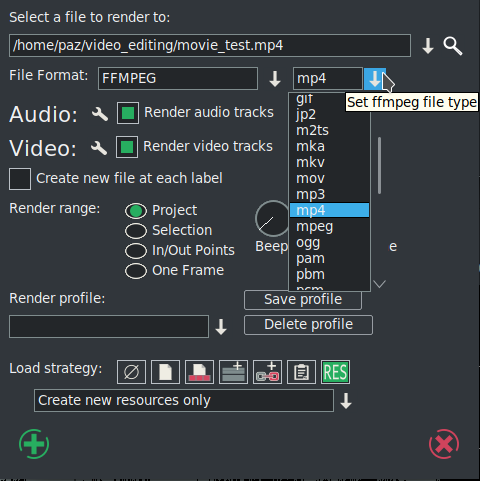
\includegraphics[width=0.7\linewidth]{images/render.png}
    \caption{Example of the Render menu}
    \label{fig:render}
\end{figure}

\begin{description}
    \item[Select a file to render to:] enter the path and filename to write the rendered file to in the textbox below.
    \item[File Format:] use the down arrow to see file format options.  For ffmpeg, which has its own set of options, you will then have to select an ffmpeg file type from the down arrow choices. The format of the file determines whether you can render audio or video or both.
    \item[Render audio tracks:] check this toggle to generate audio tracks
    \item[Render video tracks:] check this toggle to generate video tracks. The Render window will sometimes automatically update the Render Audio Tracks or Render Video Tracks checkbox as allowed by the chosen file format, but you should always check (figure~\ref{fig:render01}).  For example, if the PNG file format is selected, only the \textit{Render Video Tracks} will be checked.  Or if an ffmpeg format is chosen and the file format does not render audio, the \textit{Render Audio Tracks} will be unchecked. The invalid choices will be ghosted out.
\end{description}

\begin{figure}[htpb]
    \centering
    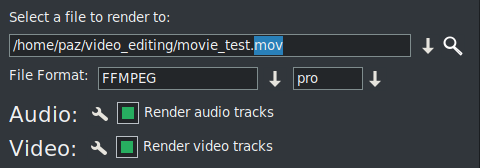
\includegraphics[width=0.7\linewidth]{images/render01.png}
    \caption{Audio and Video tracks automatically checked for Pro file type}
    \label{fig:render01}
\end{figure}

\begin{description}
    \item[Wrench:] select the \textit{wrench} next to each toggle to set compression parameters.  If the file format can not store audio or video the compression parameters will be blank.  If \textit{Render audio tracks} or \textit{Render video tracks} is selected and the file format does not support it, trying to render will result in an error message.
    \item[Create new file at each label] the option causes a new file to be created when every label in the timeline is encountered – a separate file for each.  This is useful for dividing long audio recordings into individual tracks.  When using the Render Farm (described later), \textit{Create new file at each label} causes one render farm job to be created at every label instead of using the internal load balancing algorithm to space jobs.   If the filename given in the render dialog has a 2 digit number in it, the 2 digit number is overwritten with a different incremental number for every output file. If no 2 digit number is given, Cinelerra automatically concatenates a number to the end of the given filename for every output file.
    For example, in the filename \texttt{/movies/track01.wav} the $01$ would be overwritten for every output file. 
    The filename \texttt{/movies/track.wav}; however, eventually would become \texttt{/movies/track.wav001} and so on.  
    Filename regeneration is only used when either render farm mode is active or creating new files for every label is active.
    \item[Render range:] choices are \textit{Project}, \textit{Selection}, \textit{In/Out points}, and \textit{One Frame} for single images like Tiff.  For these images, Render range will have \textit{One Frame} automatically checked and all of the others ghosted since nothing else makes sense (figure~\ref{fig:render02}).  This makes it easy to set the insertion point where you want the 1 frame to be rendered rather than having to precisely zoom in to set the in/out pointers.  Note that whichever Render range is checked, remains checked so that if \textit{One Frame} gets automatically checked, the next time you render it will still be checked and you will have to select a different one if desired.  That is why you should always check the settings.
\end{description}

\begin{figure}[htpb]
    \centering
    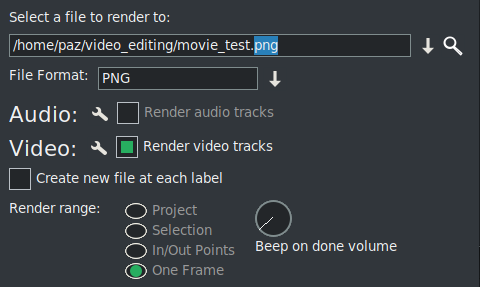
\includegraphics[width=0.7\linewidth]{images/render02.png}
    \caption{Render menu displaying a PNG \textit{one frame} option}
    \label{fig:render02}
\end{figure}

\begin{description}
    \item[Beep on done:] as a convenience when a render is complete, check this box.  It gives you the chance to work on something else while waiting and still be immediately notified when the render is complete.
    \item[Render Profile:] another convenience feature to take advantage of if you use specific render formats
    frequently, is to save that profile for future usage without having to set it up again.
    \item[Save Profile:] after setting up your render preference formats, use the save profile button to save it.
    \item[Delete Profile:] if you want to delete a saved profile, highlight the one you no longer want and delete.
    \item[Insertion strategy:] select an insertion mode from the available choices as seen when you click on the down arrow on the right hand side of the option. The insertion modes are the same as with loading files.  In the case if you select “insert nothing” the file will be written out to disk without changing the current project. For other insertion strategies be sure to prepare the timeline to have the output inserted at the right position before the rendering operation is finished. 
    
    Even if you only have audio or only have video rendered, a paste insertion strategy will behave like a normal paste operation, erasing any selected region of the timeline and pasting just the data that was rendered.  If you render only audio and have some video tracks armed, the video tracks will get truncated while the audio output is pasted into the audio tracks.
\end{description}

\section{Batch Rendering}%
\label{sec:batch_rendering}

Batch Rendering automates the rendering of audio/video files in that you can establish a set of job parameters, save them, and use them repeatedly.  It also allows for Cinelerra to be run by external programs, with no need for the user to manually interact with the user interface (figure~\ref{fig:batch01}).

If you want to render many projects to media files without having to constantly set up the render dialog for each one, batch rendering is a more efficient method of rendering.  In the Batch Render menu, you specify one or more Cinelerra project XML files, the EDL, to render and unique output files for each. (The EDL is the Edit Decision List or the set of changes to be applied to the project and media files.) Then Cinelerra loads each project file and renders it automatically. The project XML files, combined with the settings for rendering an output file, are called a batch.  This allows a large amount of media to be processed without user intervention.

\begin{figure}[htpb]
    \centering
    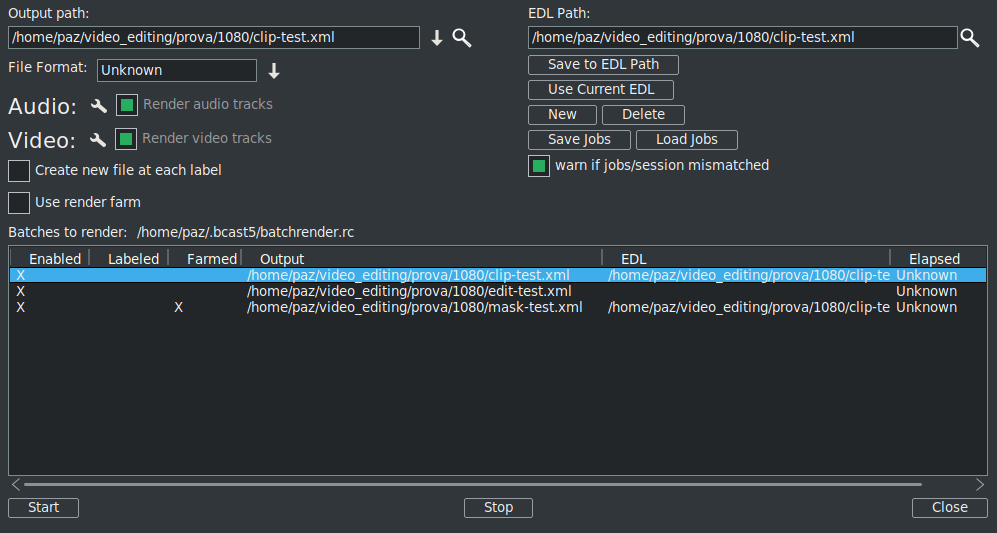
\includegraphics[width=0.8\linewidth]{images/batch01.png}
    \caption{Example of the Batch Render menu}
    \label{fig:batch01}
\end{figure}

The first thing to do when preparing to do batch rendering is to create one or more Cinelerra projects to be rendered and save them as a normal project, such as \texttt{ProjectA.xml}.  The batch renderer requires a separate project file for every batch to be rendered.  You can use the same Cinelerra project file if you are rendering to different output files, as in an example where you might be creating the same output video in different file formats.

To create a project file which can be used in batch render, set up your project and define the region to be rendered either by highlighting it, setting in/out points around it, or positioning the insertion point before it. Then save the project as usual to your \texttt{project.xm}l file. Define as many projects as needed this way.  The batch renderer takes the active region from the EDL file for rendering. If we have not set active regions, it is better to bring the insertion point to the beginning of the timeline to avoid possible problems with the rendering.

With all the Cinelerra xml project files prepared with active regions, go to \texttt{File $\rightarrow$ Batch Render}. This brings up the batch render dialog. The interface for batch rendering is more complex than for single file rendering.  A list of batches must be defined before starting a batch rendering operation.  The table of batches appears on the bottom of the batch render dialog and is called \textit{Batches to render}.  Above this are the configuration parameters for a single batch; a batch is simply a pairing of a project file with a choice of output file and render settings.

Set the \textit{Output path}, \textit{File format}, \textit{Audio}, \textit{Video}, and \textit{Create new file at each label} parameters as if you were rendering a single file.  These parameters apply to only one batch.  In addition to the standard rendering parameters, you must select the \textit{EDL Path} to be the project file (such as \texttt{ProjectA.xml}) that will be used in the batch job.  In this case, \textit{EDL Path} is not related in anyway with the EDL files as created by \texttt{File/Export EDL}.  In batch render mode the program will not overwrite an existing output file and will simply fail, so make sure that no files with the same name as the output files exist before starting.

If the batches to render list is empty or nothing is highlighted, click \texttt{New} to create a new batch. The new batch will contain all the parameters you just set.  Repeatedly press the \texttt{New} button to create more batches with the same parameters.  When you highlight any batch, you can edit the configuration on the top of the batch render window. The highlighted batch is always synchronized to the information displayed.  You can easily change the order in which the batch jobs are rendered, by clicking and dragging a batch to a different position.  Hit \texttt{Delete} to permanently remove a highlighted batch. In the list box is a column which enables or disables the batch with an \texttt{X} meaning the batch job is enabled and will be run.  This way batches can be skipped without being deleted.  Click on the \texttt{Enabled} column in the list box to enable or disable a batch.

The description of each of the columns in the batch list are as follows:

\begin{description}
    \item[Enabled:] an X in this column means the batch job will be run.
    \item[Labeled:] an \texttt{X} in this column goes hand in hand with create new file at each label.
    \item[Output:] path and filename for the generated output.
    \item[EDL:] the path and filename of the source EDL for the batch job.
    \item[Elapsed:] the amount of time taken to render the batch if finished.  If field is empty, it did not run.
\end{description}
To start rendering from the first enabled batch, hit \texttt{Start}.  Once rendering, the main window shows the progress of the batch. After each batch finishes, the elapsed column in the batch list is updated and the next batch is rendered until all the enabled batches are finished.  The currently rendering batch is always highlighted red.  To stop rendering before the batches are finished without closing the batch render dialog, hit \texttt{Stop}.  To stop rendering before the batches are finished and close the batch render dialog, hit \texttt{Close}.  Or you can exit the batch render dialog whether or not anything is being rendered, by hitting \texttt{Close}.

You can automate Cinelerra batch renders from other programs.  In the batch render dialog, once you have created your list of batch render jobs, you can click the button \texttt{Save Jobs} and choose a file to save your batch render list to.  Once you have created this file, you can start up a batch render without needing to interact with the Cinelerra user interface.  From a shell prompt, from a script, or other program, execute:

\begin{lstlisting}[language=bash,numbers=none]
    {path_to_cinelerra} -r batchjob.xml
\end{lstlisting}
substituting  your actual filename for \texttt{batchjob.xml}.  When invoked with these parameters, Cinelerra will start up and perform the rendering jobs in that list, without creating its usual windows.

\subsection{Command Line Rendering}%
\label{sub:command_line_rendering}

The command line rendering method consists of a way to load the current set of batch rendering jobs and process them without a GUI. This is useful if you want to do rendering on the other side of a low bandwidth network and you have access to a high powered computer located elsewhere. Setting up all the parameters for this operation is somewhat difficult. That is why the command line aborts if any output files already exist.

To perform rendering from the command line, first run Cinelerra in graphical mode. Go to \texttt{File $\rightarrow$ Batch Render}. Create the batches you intend to render in the batch window and close the window. This saves the batches in a file. Set up the desired render farm attributes in \texttt{Settings $\rightarrow$ Preferences} and quit out of Cinelerra if you want to use the Render Farm capability.  These settings are used the next time command line rendering is used to process the current set of batch jobs without a GUI.

On the command line run:

\begin{lstlisting}[language=bash,numbers=none]
cinelerra -r
\end{lstlisting}

\subsection{More about Save/Use EDL and Save/Load Jobs}%
\label{sub:more_save_use_edl_jobs}

The \texttt{File $\rightarrow$ Batch Render} pulldown brings up the Batch Render window to be used for batch rendering as well as DVD/BD creation.  There are some additional buttons that can save time and mistakes.  These are described next.

The \textit{Save to EDL Path} and \textit{Use Current EDL} buttons can be valuable tools for advanced usage or for developers doing testing.  Description of how you can expect them to work will help to illustrate how to take advantage of their capabilities.

\begin{description}
    \item[Save to EDL Path] if you have made a change to the EDL, use this button to save the changes so
    that they will be used in the render operation.  Although you can get the same results by using
    \texttt{File  $\rightarrow$  Save\dots}, this capability was initially added to assist developers in testing the batch jobs needed to create dvd/bluray media as it keeps the work focused in a single window and retains the original
    job name.  An example --you have everything all set up with a new job in the Batch Render window 
    using \texttt{generic.xml} for the EDL path and with a job name of \texttt{original\_name.xml}.  Then you realize
    that you forgot to cut out a section in the media that is not wanted in the final product.  You can cut 
    that out and then \textit{Save to EDL Path} so your change will be in effect for the rendering.  Without this
    button, you would be using the EDL you started with and the cut would be ignored.  Alternatively, if 
    the cut changes are saved via \texttt{File  $\rightarrow$  Save as}\dots with a filename of \texttt{new.xml} and then you use \textit{Save to EDL Path}, the current highlighted job displayed in the window as \texttt{original\_name.xml} will be 
    replaced with \texttt{new.xml}.  However, it is important to note that the result will be saved with the name
    \texttt{original\_name} – that is, the new content from \texttt{new.xml} but with the old name of \texttt{original\_name.xml}.
    \item[Use Current EDL] if you are working on media and still testing out the results, you can take
    advantage of this click-box to quickly get results.  Basically, you change the media, save that change 
    with another name (in order to preserve the original name in case you don't like the changes), and
    press \textit{Use Current EDL}.  As an example, a user creates a new job in the Batch Render window
    using the current media, previously defined in generic.xml, with the EDL path of \texttt{generic.xml}.  The
    user then changes the media on the timeline, saves the changes via \texttt{File $\rightarrow$ Save as\dots} with a new 
    name, such as \texttt{new\_name.xml}, and then clicks on \textit{Use Current EDL}.  In this case, the EDL path
    listbox will be automatically updated to the \texttt{new\_name.xml} and the current existing highlighted job will be replaced with the \texttt{new\_name.xml} in the EDL column.
    \item[Save Jobs] when you have set up the batch jobs the way you want and you think you may have to
    run them more than once, it is beneficial to save the jobs for later use so you easily run them again.
    \item[Load Jobs] reload a previous set of saved jobs.  This can come in handy if you did not have the
    time to render them when you originally set them up, if you need to rerun, or if you got interrupted.
    \item[Warn if Jobs/Session mismatched] After you set up your render and press Start, the program checks to see if the current EDL session matches your Batch Render job.  If the EDL has
    been changed since the batch job was created, it warns you so that you have the opportunity to \textit{Save to EDL} path to record those changes.  Otherwise, you can dismiss that warning box, disable the warning message by unchecking the box and use the original values.  If you never want to be warned about the mismatches, leave the box unchecked (figure~\ref{fig:batch02}).
\end{description}

\begin{figure}[htpb]
    \centering
    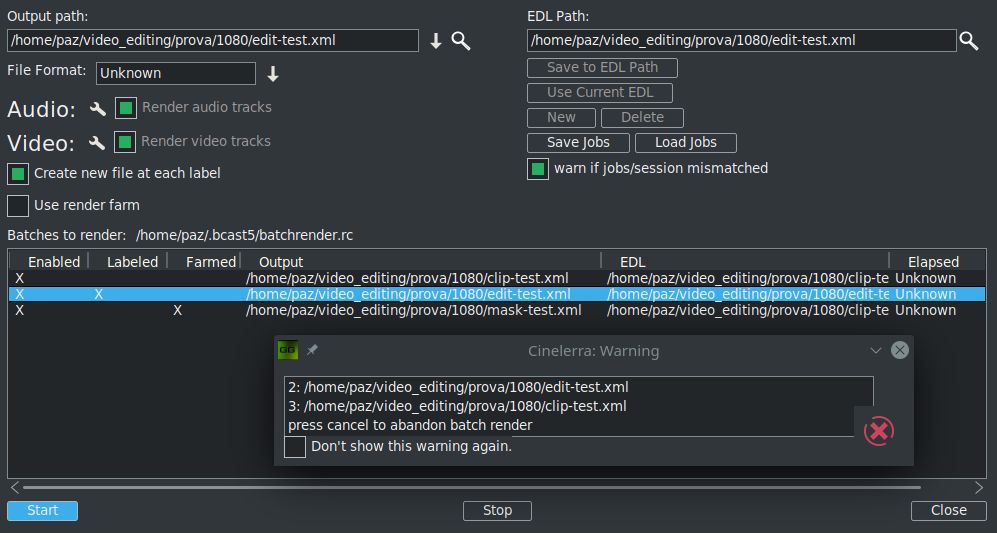
\includegraphics[width=0.8\linewidth]{images/batch02.png}
    \caption{Batch render with the 4 ghosted buttons on the right side + the Warning message below}
    \label{fig:batch02}
\end{figure}

\section{Background Rendering}%
\label{sec:background_rendering}

Background rendering causes temporary output to be rendered constantly while the timeline is being modified. The temporary output is displayed during playback whenever possible. This is useful for transitions and previewing effects that are too slow to display in real time. If a Render Farm is enabled, the render farm is used for background rendering. This gives you the potential for real-time effects if enough network bandwidth and CPU nodes exist.

Background rendering is enabled in the \texttt{Performance} tab of the \texttt{Preferences} window. It has one interactive function \texttt{Settings $\rightarrow$ Toggle background rendering}. This sets the point where background rendering starts up to the position of the insertion point. If any video exists, a red bar appears in the time ruler showing what has been background rendered (figure~\ref{fig:back-ren02}).

\begin{figure}[htpb]
    \centering
    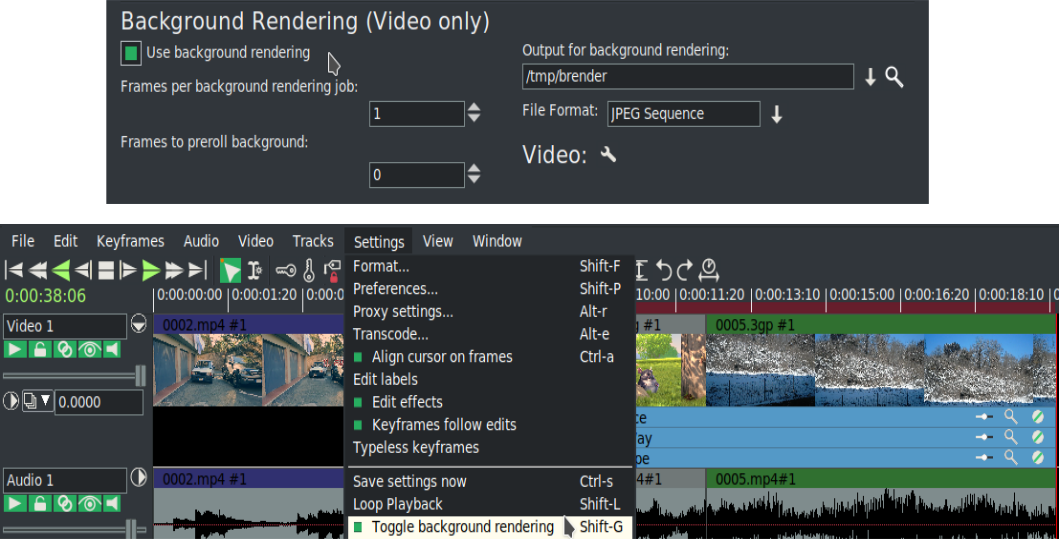
\includegraphics[width=0.8\linewidth]{images/back-ren02.png}
    \caption{Settings Background Rendering}
    \label{fig:back-ren02}
\end{figure}

It is often useful to insert an effect or a transition and then select \texttt{Settings $\rightarrow$ Toggle background rendering} right before the effect to preview it in real time and full frame rates (figure~\ref{fig:back-ren}).

\begin{figure}[htpb]
    \centering
    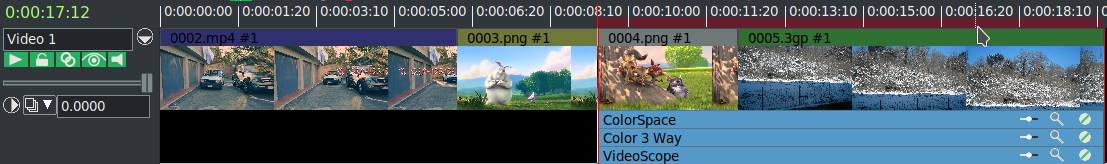
\includegraphics[width=0.8\linewidth]{images/back-ren.png}
    \caption{Timeline with the top red bar}
    \label{fig:back-ren}
\end{figure}

\begin{description}
    \item[Frames per background rendering job] This only works if a Render Farm is being used; otherwise, background rendering creates a single job for the entire timeline. The number of frames specified here is scaled to the relative CPU speed of rendering nodes and used in a single render farm job. The optimum number is 10 - 30 since network bandwidth is used to initialize each job.
    \item[Frames to preroll background] This is the number of frames to render ahead of each background rendering job. Background rendering is degraded when preroll is used since the jobs are small. When using background rendering, this number is ideally 0. Some effects may require 3 frames of preroll.
    \item[Output for background rendering] Background rendering generates a sequence of image files in a certain directory. This parameter determines the filename prefix of the image files. It should be accessible to every node in the render farm by the same path. Since hundreds of thousands of image files are usually created, ls commands will not work in the background rendering directory. The browse button for this option normally will not work either, but the configuration button for this option works.
    \item[File format] The file format for background rendering has to be a sequence of images. The format of the image sequences determines the quality and speed of playback. JPEG generally works well.
\end{description}

\section{Render Farm Usage}%
\label{sec:render_farm_usage}

Render Farm uses background rendering, a feature of Cinelerra where the video is rendered in the background, to speed up rendering significantly.  Because rendering is memory and cpu intensive, using multiple computers on a network via a render farm is a significant gain.  With Cinelerra installed on all nodes, the master node and the clients communicate via a network port that you specify. 

Cinelerra can distribute the rendering tasks over the network to the other computers of the Render Farm.  The render farm software tries to process all of the rendering in parallel so that several computers can be used to render the results.  The \textit{Total jobs to create} in the setup or labels on the timeline are used to divide a render job into that specified number of tasks.  Each background job is assigned a timeline segment to process and the jobs are sent to the various computer nodes depending upon the load balance.  The jobs are processed by the nodes separately and written to individual files.  You will have to put the files back together via a load with concatenation, or typically by using a command line tool from a script.

\subsection{Basic Steps to Start a Render Farm}%
\label{sub:basic_steps_start_render_farm}

The following steps are just a guideline to start your render farm.  It is assumed that you already have the master and client nodes communication, shared filesystem, permissions and usernames synched.

\begin{enumerate}
    \item On the master computer, use \texttt{Settings} $\rightarrow$ \texttt{Preferences} $\rightarrow$ \texttt{Performance} \texttt{tab} to set up a Render Farm:
    \begin{itemize}
        \item check the \textit{Use render farm} box;
        \item in the \textit{Hostname} box, keyin your hostname or ip address such as 192.168.1.12 or \textit{localhost};
        \item enter in a port number such as 401--405 (only a root user can use privileged ports) or $1025$  and click on \textit{Add Nodes};
        \item you will see something like the following in the Nodes listbox to the right:\newline
            \begin{tabular}{lllc}
                On & Hostname     & Port & Framerate \\\midrule
                X  & 192.168.1.12 & 401  & 0.0       \\
                X  & 192.168.1.12 & 402  & 0.0       \\
                X  & 192.168.1.12 & 403  & 0.0       \\
                X  & 192.168.1.12 & 404  & 0.0       \\
                X  & 192.168.1.12 & 405  & 0.0       \\
                X  & localhost    & 406  & 0.0       \\
                X  & localhost    & 407  & 0.0       \\
            \end{tabular}
        \item set the Total number of jobs to create;
        \item click OK on the bottom of the Preferences window.
    \end{itemize}
    \item On the client computers ($192.168.1.12$), start 5 background Cinelerra tasks via:
    \begin{lstlisting}[language=bash,numbers=none]
$ cd /{path_to_cinelerra}
$ cin -d 401
$ cin -d 402 
...
$ cin -d 405
    \end{lstlisting}
    \item On the master node (localhost), start the 2 background Cinelerra tasks via:
    \begin{lstlisting}[language=bash,numbers=none]
$ cd /{path_to_cinelerra}
$ cin -d 406
$ cin -d 407
    \end{lstlisting}
    \item When your video is ready, setup a render job via \texttt{File $\rightarrow$  Render} or \texttt{File $\rightarrow$  Batch Render} and check OK.
    \item The results will be in the shared file \texttt{path/filename} that you selected in the render menu with the
    additional numbered job section on the end as  $001, 002, 003, \dots 099$ (example, \texttt{video.webm001}).
    \item When finished, load your new files on new tracks via  \texttt{File  $\rightarrow$ Load} \textit{concatenate to existing tracks}  or if you used ffmpeg, run \textit{RenderMux} from the Shell Scripts icon.
    \item If you plan on doing more rendering, you can just leave the master/client jobs running to use again
    and avoid having to restart them.  Or you can kill them when you no longer are using them.
\end{enumerate}

\subsection{Render Farm Menu and Parameter Description}%
\label{sub:render_farm_parameter_description}

Below we describe the Performance tab for configuring a render farm (figure~\ref{fig:farm}).

\begin{figure}[htpb]
    \centering
    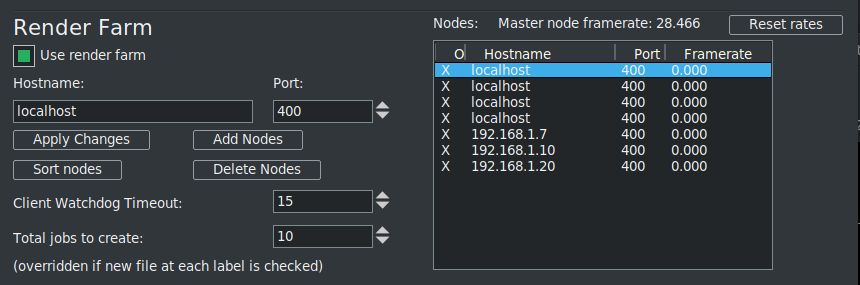
\includegraphics[width=0.8\linewidth]{images/farm.png}
    \caption{Settings $\rightarrow$ Preferences, Performance tab, menu to set up your Render Farm}
    \label{fig:farm}
\end{figure}

\begin{description}
    \item[Project SMP cpus] although this field is not Render Farm specific, it is useful for Cinelerra to have the CPU count and for using multiple threads.
    \item[Use render farm] check this to turn on the render farm option.  Once checked ALL rendering will be done via the farm including the usual Render (\texttt{Shift-R}).  You may want to turn if off for small jobs.
    \item[Nodes listbox] displays all the nodes on the render farm and shows which ones are currently enabled. The Nodes listbox has 4 columns -- On,  Hostname,  Port,  Framerate -- which show the current values.  An \textit{X} in the \textit{On} designates that that host is currently enabled; \textit{Hostname} shows the name of the host; \textit{Port} shows the port number that host uses; and \textit{Framerate} will either be zero initially or the current framerate value.
    \item[Hostname] this field is used to edit the hostname of an existing node or enter a new node.
    \item[Port] keyin the port number of an existing or new node here.  You can also type in a range of port numbers using a hyphen, for example $1501-1505$ when you need to add many.
    \item[Apply Changes] this will allow you to edit an existing node and to then commit the changes to hostname and port. The changes will not be committed if you do not click the OK button.
    \item[Add Nodes] Create a new node with the hostname and port settings.
    \item[Sort nodes] sorts the nodes list based on the hostname.
    \item[Delete Nodes] deletes whatever node is highlighted in the nodes list.  You can highlight several at once to have them all deleted.
    \item[Client Watchdog Timeout] a default value of $15$ seconds is used here and the tumbler increments by $15$ seconds.  A value of $0$ (zero) disables the watchdog so that if you have a slow client, it will not kill the render job while waiting for that client to respond.
    \item[Total jobs to create] determines the number of jobs to dispatch to the render farm.  Total jobs is used to divide a render job into that specified number of tasks.  Each background job is assigned a timeline segment to process.  The render farm software tries to process all of the rendering in parallel so that several computers can be used to render the results.  
    
    To start, if you have computers of similar speed, a good number for \textit{Total jobs to create} is the number of computers multiplied by $3$.  You will want to adjust this according to the capabilities of your computers and after viewing the framerates.  Multiply them by $1$ to have one job dispatched for every node.  If you have $10$ client nodes and one master node, specify $33$ to have a well balanced render farm.
    \item[(overridden if new file at each label is checked)] instead of the number of jobs being set to \textit{Total jobs to create}, there will be a job created for each labeled section.  If in the render menu, the option \textit{Create new file at each label} is selected when no labels exist, only one job will be created.  It may be quite advantageous to set labels at certain points in the video to ensure that a key portion of the video will not be split into two different jobs.
    \item[Reset rates] sets the framerate for all the nodes to $0$.  Frame rates are used to scale job sizes based on CPU speed of the node.  Frame rates are calculated only when render farm is enabled.
\end{description}

Framerates can really affect how the Render Farm works.  The first time you use the render farm all of the rates are displayed as $0$ in the \texttt{Settings $\rightarrow$ Preferences}, Performance tab in the Nodes box.  As rendering occurs, all of the nodes send back framerate values to the master node and the preferences page is updated with these values.  A rate accumulates based on speed.  Once all nodes have a rate of non-zero, the program gives out less work to lower rated nodes in an effort to make the total time for the render to be almost constant.
Initially, when the framerate scaling values are zero, the program just uses package length -- render size 
divided by the number of packages to portion out the work (if not labels).  If something goes wrong or the rates become suspect, then all of the rest of the work will be dumped into the last job.  When this happens, you really should \textit{reset rates} for the next render farm session to restart with a good balance.

\begin{lstlisting}[language=bash,numbers=none]
    {cinelerra pathname} -h     #displays some of the options.
\end{lstlisting}

\subsection{Detailed Setup Description}%
\label{sub:detailed_setup_description}

{\color{red} CAUTION }, any exact command lines worked as of $01/2018$ on a Fedora system.  These can change over time and on different operating systems/levels.  Always check/verify any command line before using.

\begin{description}
    \item[Set up Cinelerra] A Cinelerra render farm is organized into a master node and any number of client nodes.  The master node is the computer which is running the gui.  The client nodes are anywhere else on the network with Cinelerra installed and are run from the command line.  Before you start the master node for Cinelerra, you need to set up a shared filesystem on the disk storage node as this is the node that will have the common volume where all the data will be stored.  
    The location of the project and its files should be the same in the client computers as in the master computer and to avoid problems of permissions, it is better to use the same user in master and clients. 
    For example, if you have the project in \texttt{/home/<user>/project-video} you must create the same directory path on the clients, but empty.  Sharing the directory of the location of your project on the master computer can be done with NFS as described next.  Alternatively, you can look up on the internet how to use Samba to share a directory.
    \item[Create a shared filesystem and mount using NFS] All nodes in the render farm should use the same filesystem with the same paths to the project files on all of the master and client nodes.  This is easiest to do by setting up an NFS shared disk system.
    \begin{enumerate}
        \item On each of the computers, install the nfs software if not already installed.  For example, on Debian 9
        you will need to run: (be sure to check/verify before using any command line):
        \begin{lstlisting}[language=bash,numbers=none]
$ apt-get install nfs-kernel-server
        \end{lstlisting}
        \item On the computer that contains the disk storage to be shared, define the network filesystem.  For
        example to export \texttt{/tmp}, edit the \texttt{/etc/exports} file to add the following line:
        \begin{lstlisting}[language=bash,numbers=none]
192.168.1.0/24(rw,fsid=1,no_root_squash,sync,no_subtree_check)
        \end{lstlisting}
        \item Next reset the exported nfs directories using: 
        \begin{lstlisting}[language=bash,numbers=none]
$ exportfs -ra
        \end{lstlisting} 
        and you may have to start or restart nfs: 
        \begin{lstlisting}[language=bash,numbers=none]
$ systemctl restart nfs
        \end{lstlisting}
        \item Each of the render farm computers must mount the exported nfs target path.  To see the exports
        which are visible from a client, login as root to the client machine and keyin:
        \begin{lstlisting}[language=bash,numbers=none]
$ showmount -e <ip-addr>  #using the ip address of the storage host
        \end{lstlisting}
        \item to access the host disk storage from the other computers in the render farm, mount the nfs export on
        the corresponding target path: (be sure to check/verify before using any command line):
        \begin{lstlisting}[language=bash,numbers=none]
$ mount -t nfs <ip-addr>:/<path>  <path>
        \end{lstlisting}
        where \texttt{<path>} is the storage host directory, and \texttt{<ip-addr>} is the network address of the storage host.        
        Because all of the computers must have the same directory path, create that same directory path with the same uid/gid/permissions on each storage client computer ahead of time.
        \item To make this permanent across reboots on the client nodes, add the following line to \texttt{/etc/fstab}: 
        \begin{lstlisting}[language=bash,numbers=none]
{masternode}:/nfsshare /mnt nfs defaults 0 0
        \end{lstlisting}
        You can make this permanent on the disk storage host BUT the command lines shown, which were
        correct in January 2018 on Fedora, may be different for your operating system or in the future.  In
        addition if your network is not up, there may be numerous problems.  If you make a mistake, your
        system may not boot.  To make permanent, add the following line to \texttt{/etc/fstab}:
        \begin{lstlisting}[language=bash,numbers=none]
192.168.1.12:/tmp /tmp nfs rw,async,hard,intr,noexec,noauto 0 0
        \end{lstlisting}
        You will still have to mount the above manually because of the \textit{noauto} parameter but you won’t
        have to remember all of the other necessary parameters.  Depending on your expertise level, you can
        change that.
        
        Later, to remove access to the storage host filesystem:        
        \begin{lstlisting}[language=bash,numbers=none]
$ umount <path>
        \end{lstlisting}
        
        Be aware that you may have to adjust any security or firewalls you have in place.  \textit{Most firewalls will require extra rules to allow nfs access}.  Many have built-in configurations for this. 
    \end{enumerate}
    \item[Configure Rendering on Master Node] There is 1 master node which is running the Cinelerra gui and where the video will be edited and the command given to start up the rendering.  Any number of client computers can be run from the command line only, so they can be headless since no X or any graphical libraries are needed.  Of course, the Cinelerra software must be installed on each of the client computers.
    \begin{enumerate}
        \item Assuming you already have Cinelerra installed on the master node, start Cinelerra by clicking on the
        icon or by typing the following command on the terminal screen:  \texttt{/{cinelerra\_path}/cin}.
        \item Use the file pulldown \texttt{Settings $\rightarrow$ Preferences}, the Performance tab, to set up your Render Farm
        options in the Render Farm pane.
        \item Check the \textit{Use render farm} option.  By default, once you enable the option of Render Farm, rendering is usually done using the render farm.  Batch rendering can be done locally, or farmed.
        \item Add the hostname or the IP address of each of the client nodes in the Hostname textbox and the port
        number that you want to use in the Port textbox.  You can make sure a port number is not already in
        use by keying in on the command line:
        \begin{lstlisting}[language=bash,numbers=none]
$ netstat -n -l -4 --protocol inet
        \end{lstlisting}
        Next, click on the \textit{Add Nodes}
        button and then you will see that host appear in the Nodes list box to the right.  The \texttt{X} in the first
        column of the nodes box denotes that the node is active.  To review the \textit{standard} port allocations,
        check the \texttt{/etc/services} file.
        \item Enter the total jobs that you would like to be used in the \textit{Total job} textbox.
        \item The default watchdog timer initial state is usually just fine but can be adjusted later if needed.
        \item Click OK on the Preferences window when done.
    \end{enumerate}
    \item[Create Workflow] While working on the master computer, it is recommended that you keep all the resources being used on the same shared disk.  Load your video/audio piece and do your editing and preparation.  Add any desired plugins, such as a Title, to fine-tune your work.  You want to make sure your video is ready to be rendered into the final product.
    \item[Start the Client Nodes] To start up the client nodes run Cinelerra from the command line on each of the client computers using the following command:
    \begin{lstlisting}[language=bash,numbers=none]
/{cinelerra_pathname}/cin -d [port #]   ;   \#for example /mnt1/bin/cinelerra -d 401
    \end{lstlisting}
    This starts Cinelerra in command prompt mode so that it listens to the specified port number for commands from the master node for rendering.  When you start each of the clients up, you will see some messages scroll by as each client is created on that computer, such as:
    \begin{lstlisting}[language=bash,numbers=none]
RenderFarmClient::main_loop: client started
RenderFarmClient::main_loop: Session started from 127.0.0.1
    \end{lstlisting}
    As it completes its jobs, you will should see:
    \begin{lstlisting}[language=bash,numbers=none]
RenderFarmClientThread::run: Session finished
    \end{lstlisting}
    A quick way to start a sequence of clients is to use:
    \begin{lstlisting}[language=bash,numbers=none]
or n in `seq 1501 1505`; do cin -d $n; done
    \end{lstlisting}
    \item[Render Using Render Farm] After you have followed the preceding steps, you are ready to use the render farm.  Click on \texttt{File $\rightarrow$ Render}\dots which opens the render dialog.  The most important point here is to use for \textit{the Output path / Select a file to render to} a path/file name that is on the shared volume that is also mounted on the clients.  Click on OK to render. The Cinelerra program divides the timeline into the number of jobs specified by the user.  These jobs are then dispatched to the various nodes depending upon the load balance. The first segment will always render on the master node and the other segments will be farmed out to the render nodes.  Batch Rendering, as well as BD/DVD rendering, may use the render farm.  Each line in the batchbay can enable/disable the render farm.  Typically, video can be rendered into many file segments and concatenated, but normally audio is rendered as one monolithic file (not farmed).
    
    Another performance feature which can use the Render Farm is \textit{Background Rendering}.  This is also enabled on the \texttt{Preferences $\rightarrow$ Performances} tab.  The background render function generates a set of image files by pre-rendering the timeline data on the fly.  As the timeline is update by editing, the image data is re-rendered to a \textit{background render} storage path.  The Render Farm will be used for this operation if it is enabled at the same time as the \textit{background render} feature.
    \item[Assemble the Output Files] Once all of the computer jobs are complete, you can put the output files together by using the shell script, \textit{RenderMux} (from the menubar \textit{scripts} button just above FF), if the files were rendered using ffmpeg, or you can load these by creating a new track and specifying concatenate to existing tracks in the load dialog in the correct numerical order.  File types which support direct copy can be concatenated into a single file by rendering to the same file format with render farm disabled as long as the track dimensions, output dimensions, and asset dimensions are equal.
\end{description}

\subsection{Quick and Easy Render Farm Setup – The Buddy System Way}%
\label{sub:buddy_system_way}

These steps are for quickly setting up render farm with the least amount of additional system work, but it is non-optimal.  It is useful in situations where a few people all show up with their laptops to work together on the same video/audio file and you don’t want to bother setting up NFS for a shared disk.

\begin{enumerate}
    \item Make sure the Cinelerra program is installed on all of the computers and the network between the
    main computer and the client computers is working.  Use the same version if possible.
    \item Load your video file on the master node and use \texttt{File $\rightarrow$ Save as}\dots  to save it to \texttt{/tmp}.
    \item Move that same file with the same name to \texttt{/tmp} on all of the client computers via rsh or sneaker net -- the ONLY reason you are doing this is to avoid having to set up NFS or Samba on the buddy client
    laptops that show up!
    \item Edit your video/audio file to get it the way you want it and add the plugins, such as a Title, etc.
    \item Check for a set of unused ports in \texttt{/etc/services} file, if username is root usually $401-425$ are
    available; if non-root, then $1024-1079$.
    \item On the master computer, in \texttt{Settings $\rightarrow$ Preferences, Performance} tab:
    \begin{itemize}
        \item check the box \textit{Use render farm}
        \item keyin localhost for the hostname or an ip address of the buddy client node
        \item keyin the desired port number for each client; and use \textit{Add Node} for each host
        \item set total jobs to the number of client computers $+1$ multiplied by $3$ (or proportion to client speeds)
        \item check OK
    \end{itemize}
    \item On each buddy client, create a job for each port:    
    \begin{lstlisting}[language=bash,numbers=none]
/{cinelerra_pathname}/cin -d port#
    \end{lstlisting}
    \item On the master, bring up the render menu and name the output files, for example \texttt{/tmp/myoutput.mp4}.
    \item The client nodes output results will be on their local \texttt{/tmp} filesystems so you will have to again use
    \textit{rsh/ftp} or \textit{usb sneaker net} to move them over to the main computer.  File names will be the render
    job output file name with port number tacked on (e.g. \texttt{/tmp/hb.mp4001...mp4005}).
    \item Load the files by concatenate to existing track on the master node or use RenderMux shell script.
\end{enumerate}

\subsection{Multi-core Computers Render Farm Setup\protect\footnote{the 'Epyc' method}}%
\label{sub:multi_core_render_farm_setup}

Because index files speed up displaying the video you may want to share these files with the clients on a shared filesystem.  There is a configuration option available in \texttt{Settings $\rightarrow$ Preferences}, the Interface tab, that sets up in your preferences the location of the index files which you can put on a shared disk.
Screencast below shows part of the Preferences menu where you can change the index files setup (figure~\ref{fig:index}).
\begin{figure}[htpb]
    \centering
    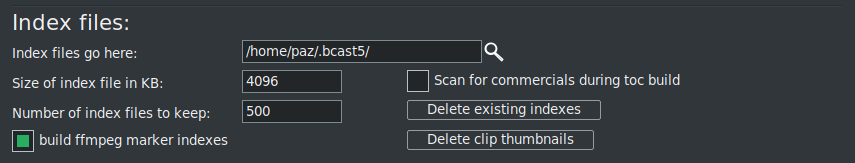
\includegraphics[width=0.8\linewidth]{images/index.png}
    \caption{Index file setup for your preferred configuration for Render Farm sharing or anything}
    \label{fig:index}
\end{figure}
 Or, one of the convenient features of cin5 is the redirection of the path via \texttt{CIN\_CONFIG} as in:
\begin{lstlisting}[language=bash,numbers=none]
CIN_CONFIG=/<shared_file_pathname>/<filename_such_as_.bcast5> /<cinelerra_pathname>/cin
\end{lstlisting}
This means that you can make project related configurations that do not impact the default \texttt{\$HOME} config.  You can either export your default \texttt{\$HOME} config or the \texttt{CIN\_CONFIG} config to use on the render farm.

\subsection{Troubleshooting Tips and Warnings}%
\label{sub:troubleshhoting_tips_warnings}

\noindent If you have problems running the Render Farm.  Here is a list of items to check.

\begin{itemize}
    \item Cinelerra must be installed on the master node and all client machines.
    \item It is best to have the same username available on all nodes to avoid problems with access rights.
    \item Check file permissions and ownership to ensure that the clients all have access.
    \item If a node does not have access to an input asset it will not die, but just display error messages.
    \item If a node can not access an output asset, the rendering will abort.
    \item A port in use when stopped may take up to $30$ seconds to time out before you can restart the jobs.
    \item Each of the port combinations have to be unique across clients, and not already in use in the network.
    \item Cinelerra load balances on a first come, first serve basis.  If the last section of the video is sent to the
    slowest node, the render job will have to wait for the slowest node to finish.  It would be better to 
    start on the slowest node with the earlier section of the video so keep that in mind when designating
    port numbers.
    \item If not running as root, a port number in the higher range of $1024$ and above must be used instead of
    the $400+$ range.
    \item The master and client jobs on the ports do not go away so if you want to stop them, you will have to
    kill them via: \texttt{kill PID\#}.
    \item Check to see if there are services listening on the ports to use:  \texttt{netstat -n -l -4 --protocol inet}
    \item There is a watchdog timer in Cinelerra and if there is no response from a client in the designated
    number of seconds, it will kill the render job.
    \item The \textit{localhost} should exist as $127.0.0.1$ in \texttt{/etc/hosts} and as the \texttt{lo} network device in ifconfig.
    \item If the job loads become unbalanced, you may want to \textit{reset rates} to start over for new framerates.
    \item If jobs are split in a key section on the timeline, you may wish to \textit{use labels} to prevent this.
    \item For testing purposes, you may want to start a client in the foreground using \texttt{-f} instead of \texttt{-d}.
    \item If one of the client computers is unavailable, check to see if there is an \texttt{X} to the left of the \texttt{nodename}
    in the Nodes listbox.  Check the \texttt{X} to disable it which sets ON to OFF.
    \item A red message in the lower left hand corner of the main timeline that reads \textit{Failed to start render
    farm} often means that the client Cinelerra programs were not started up.
    \item A message of \texttt{RenderFarmWatchdog::run 1 killing server thread \\ \#address\#} means that the client did
    not respond in time.  You can adjust the timer in \texttt{Settings $\rightarrow$ Preferences, Performance} tab.
    \item When you get the message \texttt{RenderFarmClient::main\_loop: bind port 400: Address already in use}, use a different port.
    \item A message of \texttt{RenderFarmServerThread::open\_client: unknown host abcompany} means that the
    hostname of abcompany is not in \texttt{/etc/hosts} so you will have to add it or use the ip address instead.
    \item There are numerous error messages associated with file \textit{open/close/status} or problems with the file
    that should be dealt with according to what is printed out.
    \item Other illustrative messages may be shown such as: \texttt{RenderFarmClientThread:: run: Session finished}.
\end{itemize}

\paragraph{Warnings}

If one of the render farm computers is connected to the internet, you should use a firewall to maintain the safety of all of the computers.  The ports have to be reachable for the intranet but you do not want the ports to be open to the outside.

\section{Some Specific Rendering}%
\label{sec:some_specific_rendering}

\noindent The next few pages relate to rendering for specific common cases.

\subsection{FFmpeg Common H.264 Rendering}%
\label{sub:ffmpeg_h264_rendering}

Because H.264 is so widely used, the method in Cinelerra-GG Infinity is outlined below.  These setup steps make it easy to just get started.

\begin{itemize}
    \item File $\rightarrow$ Render
    \item File Format $\rightarrow$ FFMPEG + mp4
    \item Video Wrench $\rightarrow$ Preset $\rightarrow$ h264.mp4 + bitrate: 6000000 (or whatever) + OK
    \item Audio Wrench $\rightarrow$ Preset $\rightarrow$ h265.mp4 + bitrate: 224000 (or whatever) + OK
    \item Set your target path in: Render $\rightarrow$ Select a file to render to
    \item Set your timeline in: Render $\rightarrow$ Render range + click Project
    \item Set your insertion strategy: Replace project (or whatever)
    \item Press OK to start rendering.
\end{itemize}

\subsection{Lossless Rendering}%
\label{sub:loseeless_rendering}

Lossless means that in the compression of a file, all of the original data, every single bit, can be recovered when the file is uncompressed.  This is different than \textit{lossy compression} where some data is permanently deleted so that when uncompressed, all of the original data can not be exactly recovered.  Lossy is generally used for video and sound, where a certain amount of information loss will not be detected by most users or the playback hardware does not reproduce it anyway -- it is a trade-off between file size and image/sound quality.  The files created will be more than 10 times larger than usual.  Most players will not be able to decode lossless as the bitrate will overwhelm the device.

For x264 lossless compression to work, the only color model allowed here is yuv420p.  Any other specification will be converted to yuv420p and the data will be modified.  Also, keep in mind that the YUV color model has to be converted to RGB, which also modifies the data.

To use x264 lossless rendering -- choose File format of ffmpeg, m2ts in the Render window.  Click on the Video wrench, which brings up the Video Preset window and scroll down in the Compression filebox and choose \texttt{lossless.m2ts}.  \textit{Preset=medium} is the default, but can be varied from \textit{ultrafast} (least amount of compression, but biggest file size) to \textit{veryslow} (most amount of compression, but still HUGE) in the parameter box where you see $qp=0$.  This option is also available for bluray creation.

\subsection{Extra “cin\_” Options for Render with FFmpeg}%
\label{sub:extra_cin_option_ffmpeg}

There are several special parameters that can be used in the ffmpeg options file to pass values to the codecs that are not normally available.  These are explained below.

\paragraph{cin\_pix\_fmt} The Render menus allows you to choose the codec input pixel format (figure~\ref{fig:yuv420}).  The Pixels selection provides the available pixel format options for the chosen codec type; valid choices vary for the different file types.  This list represents the formats that the codec advertises.  It is not always complete, and it may include options that are not legal with all parameter configurations.

\begin{figure}[htpb]
    \centering
    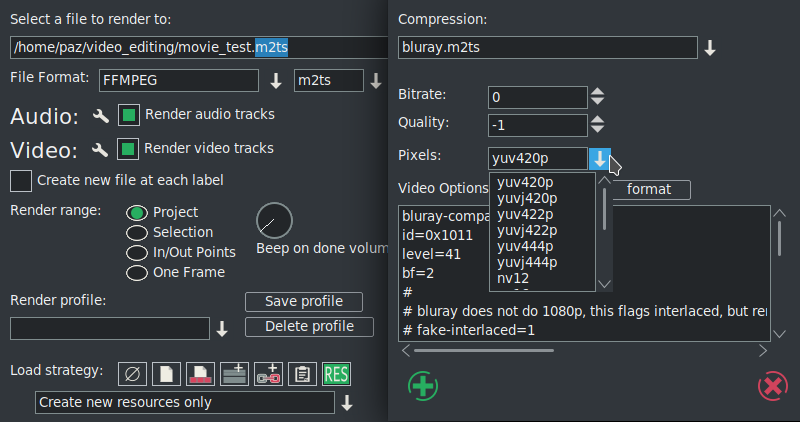
\includegraphics[width=0.6\linewidth]{images/yuv420.png}
    \caption{Render \& Video Preset menus displaying Pixel choices}
    \label{fig:yuv420}
\end{figure}

\begin{itemize}
    \item The \textit{Bitrate}, \textit{Quality}, and \textit{Pixels} fields are only updated when the Video Options are reloaded.  This
    occurs when you either change the ffmpeg file format, or video presets compression fields.
    \item If the video options preset has \textit{cin\_pix\_fmt} defined, its value will be loaded as the default.  If you
    override the default, the value you specify will be used.
    \item If the video options preset does not have \textit{cin\_pix\_fmt}, the default pixel format will be computed by ffmpeg (\textit{avcodec\_find\_best\_pix\_fmt\_of\_list}), using the session format as the source choice.  The
    \textit{best} is usually the format which is most similar in color and depth.
    \item If no choices are available, yuv420p for video will be used.
    \item You can also specify ffmpeg pixel formats which are not in the list.  The list is provided by ffmpeg as input selection, but is more like suggestions than fact.  For example, the raw formats can take almost any format, but the rawvideo codec actually specifies no legal formats.
\end{itemize}

\noindent Some option files provide \textit{cin\_pix\_fmt} to suggest a choice for good quality output or to prevent parameter errors when the other provided parameters conflict with the \textit{best} pixel format.  This is the case in \texttt{faststart\_h264.mp4} where the \textit{profile=high} parameter dictates pixel format must be \texttt{yuv420p}.

\paragraph{cin\_bitrate} If you specify the bitrate, you can not specify the quality.\\
Example: \textit{cin\_bitrate=2000000}

\paragraph{cin\_quality} If you specify the quality, you can not specify the bitrate.\\
Example: \textit{cin\_quality=7}

\paragraph{cin\_stats\_filename} This parameter is useful for 2 pass operations.\\
Example: \texttt{cin\_stats\_filename /tmp/cin\_video\_vp9\_webm}

\paragraph{cin\_sample\_fmt} For audio the preset sample format default is computed in a similar way as stated above for video or can be set with the \textit{cin\_sample\_fmt} parameter (figure~\ref{fig:audio}).  If no choices are provided, s16 will be used.\\
Example: \textit{cin\_sample\_fmt=s16}

\begin{figure}[htpb]
    \centering
    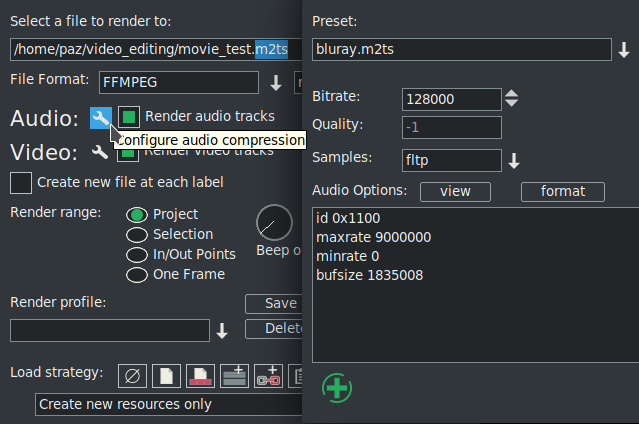
\includegraphics[width=0.55\linewidth]{images/audio.png}
    \caption{Render menu showing where Samples is}
    \label{fig:audio}
\end{figure}

\subsection{Two-pass Encoding with FFmpeg}%
\label{sub:two_pass_encoding_ffmpeg}

In Cinelerra for two-pass, you need to run ffmpeg twice, with the same settings, except for designating the options of pass 1 for the first pass and then pass 2.  In pass 1, a logfile that ffmpeg needs for the second pass is created.  In pass 1 the audio codec should be specified that will be used in pass 2.  For more information on ffmpeg 2-pass, check {\small \url{https://trac.ffmpeg.org/wiki/Encode/H.264}}.  Different libraries may have different requirements and you will probably have to determine this by looking online at ffmpeg or looking directly at that code.

This 2 line ffmpeg 2-pass operation can be functionally duplicated in Cinelerra in the steps below them:

\begin{lstlisting}[language=bash,numbers=none]
ffmpeg -y -i input -c:v libx264 -b:v 2600k -pass 1 -c:a aac -b:a 128k -f mp4 /dev/null && \
ffmpeg -i input -c:v libx264 -b:v 2600k -pass 2 -c:a aac -b:a 128k output.mp4
\end{lstlisting}

\begin{enumerate}
    \item After you have completed your editing, do a Save Session with \texttt{File $\rightarrow$ Save as}\dots
    Before starting, be sure your session is ready for batch render. That is, positioned at the beginning and nothing selected.
    \item Bring up \texttt{File $\rightarrow$ Batch Render}\dots where you will do the setup.
    \item Click on the \textit{Delete} box  to remove old jobs highlighted in the bottom listbox.
    \begin{itemize}
        \item For the \textit{File Format} choose ffmpeg and mp4 for the type.
        \item Set \textit{Output path} to the path and filename for the render output file.
        \item Click on \textit{Use Current EDL} to use the designated EDL Path file.
        \item Click on \textit{New} and you will see a new highlighted job show up in the listbox at the bottom.
        \item Use the Audio wrench to set bitrate to $128000$ ($128k$ as in ffmpeg example above).
        \item Click checkmark OK.  Open the video tools with the video wrench.
        \item Set the Video Compression to \textit{h264.mp4} (as seen in the example).
        \item Set the bitrate to $2600000$ ($2600k$ as in ffmpeg example above).
        \item Add the following 2 lines after the first line:
        \begin{lstlisting}[language=bash,numbers=none]
flags +pass1
passlogfile /tmp/{temporary log file name}.log
        \end{lstlisting}
        Click checkmark OK.
    \end{itemize}    
    \item Click on \textit{New} to create the second pass job.  You will see this second job in the listbox below.
     Use the Video wrench and change pass1 to pass2 as follows.
        \begin{lstlisting}[language=bash,numbers=none]
flags +pass2
        \end{lstlisting}
    \item Click checkmark OK.
    \item Click on the \textit{Start} box and watch it go!
    \item You can now check the output file for results.  At the time this was documented, \textit{rc=2pass} will be
        in the output.    
\end{enumerate}

If you need to re-render this, the Batch Render will still be set up but you have to click on the \textit{Enabled} column in the listbox to re-enable the jobs to run which puts an X there.  Click Start again. You can reuse batch job using the \textit{save jobs} and \textit{load jobs} buttons in the batch render dialog.

\paragraph{Render shortcuts for webm, h264, h265} are available by using the option files that are already set up for this purpose.  Use the render menu as usual, with ffmpeg/mp4, choose h264 or h265 \textit{pass1of2\_h26x} for the video and \textit{passes1and\-2\_h26x} for the audio; 
with ffmpeg/webm, choose \textit{pass1of2\_vp9}.  When that is finished, you will have to use the render menu again and this time for video, choose \textit{pass2of2\_h26x} or \textit{pass2of2\_vp9}.  The logfile is hard coded in the options file so will write over any currently existing logfile if you do not change it before you start the render.

\paragraph{Requirements for some other libraries} ~\\ (used instead of \textit{flags +pass1} \& \textit{passlogfile}):

\begin{description}
    \item[x265:] add this line:
    \begin{lstlisting}[language=bash,numbers=none]
x265-params=pass=1:stats=/tmp/{temporary log file name}.log
    \end{lstlisting}      
    at the time this document was written, you should see in the output: \\  \textit{stats-read=2}
    
    \item[libvpx-vp9, xvid, and huffyuv:]~

    \begin{lstlisting}[language=bash,numbers=none]
    cin_stats_filename /tmp/{temporary log file name}.log
    flags +pass1 (or flags +pass2 for the second pass)
    \end{lstlisting}    
\end{description}

\textit{NOTE:} for vp9, the best Pixels is \textit{gbrp}

\subsection{Use case: High Efficiency Video Coding (HEVC)}%
\label{sub:use_case_hevc}

An example of video profile based on CRF, a quality-controlled
variable bitrate, instead of fixed quality scale (ABR).
HEVC (H.265) was developed as a successor to AVC (H.264) to more
efficiently compress the future large amounts of data from 2/4/8k
videos.
In comparison to AVC, an average saving of around 30 percent can be
assumed for the same quality.
Because HEVC is not bound to any size format, it is suitable for
virtually any image size.

The following example is HD and FullHD oriented and produces a
picture quality similar to the Blu-ray with some limitations.
As container Matroska (\texttt{.mkv}) is used, but also mp4 and others are
possible.

\vspace{2ex} \begin{lstlisting}[language=bash,numbers=none]
matroska libx265

# CRF 16 creates a balanced compromise
# between quality and file size. 
crf=16

# Preset changes encoding speed and generally
# degrades the overall result. Medium (default)
# always fits.
preset=medium

# Additional parameters that are passed on to the codec.
# me=star improves the search for very fast
# movements, but slows down the encoding.
#x265-params=me=star

# Keyint does FFmpeg automatically, otherwise
# the setting must match the frame rate.
#keyint\_min=25

# Profile does FFmpeg automatically.
#profile=high

# Source sRBG and retention of color space.
# 720/1080=bt709 if no profile set. Useful
# for formats smaller than 720 if no lossy
# conversion is desired.
colorspace=bt709
color_trc=bt709
color_primaries=bt709

# Output in 10 bit, prevents 8-bit step formation
pixel_format=yuv420p
\end{lstlisting}

\noindent \textit{NOTE:}

A CRF of 16 delivers satisfactory results in most cases. However, if
the video material is really \emph{grainy}, a CRF~16 can lead to unwanted large files.  In this case, a trial export of perhaps one minute should be performed. The resulting bit rate can be used to correct the CRF to 17,\,18,\,19\ldots -- remember, a CRF of 0 means lossless, the higher the number the stronger the lossy compression. The approximate calculation of the final file size can be extrapolated from the sample export.

The color space information must be used explicitly so that it can
be included in the video. Cinelerra\,GG or FFmpeg does not write it
by itself. Without this information the players (e.\,g.\ \href{https://mpv.io/}{mpv}) stick to the dimensions of the video and take the assumed color model from a table. With videos in the dimensions from 720 to 1080 this is bt709. For smaller dimensions, e.\,g.\ DVD, bt601 is assumed and for 4k and above it is bt2020. Normally this is not a problem, but if you want to export a FullHD without color loss to a smaller size like 576 for example, you have to inform the encoder as well as the decoder of the player. This also applies if the videos are to be loaded on video platforms, where they are then converted into videos of different sizes. It is a security measure to prevent false colors, such as the color profiles in digital photos and the copies made from them.

The HEVC tuning has not been considered here, because it is is
rarely used and requires background knowledge.

Further links:
\begin{itemize}
    \item \href{http://x265.readthedocs.org/en/default/}{x265
        Documentation}
    \item \href{http://x265.readthedocs.org/en/latest/cli.html}{x265
        Command Line Options}
    \item \href{http://x265.readthedocs.org/en/latest/presets.html}{x265
        Presets/Tuning}
\end{itemize}

\subsection{Piping Video to a Command Line}%
\label{sub:piping_video_command_line}

You can pipe a video to any command line on the computer, such as ffmpeg.  This can be especially useful with raw video files.  Next is an example usage.

\begin{enumerate}
    \item on a terminal window create a named pipe file, for example:
    \begin{lstlisting}[language=bash,numbers=none]
mknod /tmp/piper.yuv p
    \end{lstlisting}
    load your video and do your editing
    \item set up your Render (\texttt{Shift-R}), you can choose a raw format such as \textit{yuv} or \textit{rgb}
    \item for the filename \textit{Select a file to render to}, use the named pipe as created in step 1 (\texttt{/tmp/piper.yuv})
    \item for \textit{Insertion Strategy}, you will want to make sure to select \textit{insert nothing}
    \item click for OK on the green checkmark.(the Cinelerra gui will look like it is hanging while waiting for a command line to use the pipe.)
    \item on the terminal window, keyin your command, for example:
    \begin{lstlisting}[language=bash,numbers=none]
/mnt0/build5/cinelerra-5.1/thirdparty/ffmpeg-3.4.1/ffmpeg -f rawvideo -pixel_format yuv420p \ -video_size 1280x720 -framerate 30000/1001 -i /tmp/piper.yuv /tmp/pys.mov
    \end{lstlisting}
\end{enumerate}

A slightly different option can be used instead that may be more familiar to some.  In the render menu after choosing the File Format of \textit{ffmpeg}, use the pulldown to choose \textit{y4m} as the file type.  This choice results in putting a header on the rendered output with some pertinent information that can be used for ffmpeg processing thus alleviating the requirement for \textit{pixel\_format}, \textit{video\_size}, and \textit{framerate} on the ffmpeg command line.  In this case the format is \textit{yuv4mpegpipe} instead of \textit{rawvideo}.  An example command line would look as follows (assuming the created pipe is called \texttt{piper.y4m}):
\begin{lstlisting}[language=bash,numbers=none]
ffmpeg -f yuv4mpegpipe -i /tmp/piper.y4m -vcodec libx264 /tmp/test.mp4
\end{lstlisting}

\subsection{Faststart Option for MOV type files}%
\label{sub:faststart_option_mov0}

If you have mov video and want to be able to start playing without having to first load the entire video, \textit{-movflags=+faststart} is needed for ffmpeg to put the meta-data, known as the \textit{moov atom}, at the beginning of the file.  Otherwise, ffmpeg puts this atom at the end of the video file which means you have to wait to play until the whole video is loaded.  Or worse yet, if the file becomes damaged in the middle and you can not get to the end, you won’t be able to play anything.

Now you can have the \textit{moov atom} put on the front of the file (automatically via a second pass).  To do this, when rendering using ffmpeg \& either the mp4 or qt format/container, click on the video/audio wrenches and choose \textit{faststart\_h264}.   With the \textit{qt} format, settings will just be the default whereas the \textit{mp4} format uses the highest quality and lowest file size as possible, but you can easily modify these options in the associated Video Preset textbox.

